% !TeX spellcheck = en_US
\documentclass[aspectratio=1610]{beamer}
\mode<presentation>
{
  \usetheme{Boadilla}
  \setbeamercovered{transparent}
  
  \definecolor{cobalt}{rgb}{0.0, 0.02 0.50}
  
  \usecolortheme[named=cobalt]{structure}
  %\usecolortheme{lily}
  %\setbeamercolor{headline}{fg=cyan!80!black}
  % \setbeamercolor{frametitle}{bg=white}.
}

\makeatletter
\define@key{beamerframe}{wide}[10pt]{%
	\def\beamer@cramped{\itemsep #1\topsep0.5pt\relax}}
\makeatother
	

\usepackage[english]{babel}
\usepackage[utf8]{inputenc}
\usepackage{times}
\usepackage[T1]{fontenc}
\usepackage{array}
\usepackage{xcolor}
\usepackage{colortbl}
\usepackage{booktabs}

\title[Fall - Lecture 8] % (optional, use only with long paper titles)
{Macroeconomic Theory and Policy: Lecture  8 (Ch.6)}

\author[University of Toronto] % (optional, use only with lots of authors)
{}
\date[] % (optional, should be abbreviation of conference name)

\begin{document}

\begin{frame}
  \titlepage
\end{frame}

%\begin{frame}[wide]{Population Growth in the Solow Model}
%	\begin{itemize}
%		\item Recall the capital accumulation function:
%		\[K_{t+1} = K_{t} + I_t - \delta K_t\]
%		\item Divide both side by $L_t$
%		\[\frac{K_{t+1}}{L_t} = \frac{K_{t}}{L_t} + \frac{I_t}{L_t} - \delta \frac{K_t}{L_t}\]
%		All the term on the RHS can easily convert into per capita term, but on the LHS, the capital in period $t+1$ is not divided by the population size in the same period
%		\item Rearrange the population growth formula: $L_t = \frac{L_{t+1}}{1+n}$ and sub it into the LHS
%		\[\frac{K_{t+1} }{L_{t+1}} (1+n) = \frac{K_{t}}{L_t} + \frac{I_t}{L_t} - \delta \frac{K_t}{L_t}\]
%		\item Now, we can convert all variables into per capita term
%		\[k_{t+1} (1+n) = k_t + i_t - \delta k_t\]
%	\end{itemize}
%\end{frame}

\begin{frame}[wide]{Population Growth in the Solow Model}
	\begin{itemize}
		\item As observed from the data, population growth is a significant contributor to total GDP growth.
		\begin{itemize}
			\item For example, by simple decomposition, population growth in the U.S. accounts for 1.5\% of the total 3.5\% GDP growth.
		\end{itemize}
		\item Including population growth in the Solow model is important for studying total GDP growth.
		\item Assume population grows at a constant rate:
		\[
		L_{t+1} = (1 + \bar{n}) L_t
		\]
		\begin{itemize}
			\item \(\bar{n}\) represents the constant rate of population growth.
		\end{itemize}
	\end{itemize}
\end{frame}

\begin{frame}[wide]{Population Growth in the Solow Model}
	\begin{itemize}
		\item Recall the capital accumulation equation:
		\[
		\Delta k_{t+1} = \bar{s} y_t - \delta k_t
		\]
		\item Dividing both sides by \(k_t\):
		\[
		\frac{\Delta k_{t+1}}{k_t} = \bar{s} \frac{y_t}{k_t} - \delta
		\]
		\item The term \(\frac{\Delta k_{t+1}}{k_t}\) represents the growth rate of capital per capita.
		\item Recall \(k_t = \frac{K_t}{L_t}\), so \(g_k = g_K - g_L\):
		\[
		\frac{\Delta k_{t+1}}{k_t} = \frac{\Delta K_{t+1}}{K_t} - \frac{\Delta L_{t+1}}{L_t} = \frac{\Delta K_{t+1}}{K_t} - \bar{n}
		\]
	\end{itemize}
\end{frame}

\begin{frame}[wide]{Population Growth in the Solow Model}
	\begin{itemize}
		\item The capital accumulation function at the aggregate level can be rearranged as:
		\[
		\frac{\Delta K_{t+1}}{K_t} = \bar{s} \frac{Y_t}{K_t} - \delta = \bar{s} \frac{y_t L_t}{k_t L_t} - \delta = \bar{s} \frac{y_t}{k_t} - \delta
		\]
		\item Substituting this into the formula from the previous slide:
		\[
		\frac{\Delta k_{t+1}}{k_t} = \bar{s} \frac{y_t}{k_t} - \delta - \bar{n}
		\]
		\item Multiplying both sides by \(k_t\):
		\[
		\Delta k_{t+1} = \bar{s} y_t - (\delta + \bar{n}) k_t
		\]
		\item Compared to the baseline model, investment must not only cover capital depreciation but also provide new capital for the growing population.
	\end{itemize}
\end{frame}

\begin{frame}[wide]{Population Growth in the Solow Model}
	The Solow diagram remains similar to the baseline model, except that the depreciation curve is steeper due to the additional term \(\bar{n}\).
	\begin{figure}
		\centering
		\includegraphics[width=0.7\linewidth]{"Figures/MACRO6_FIG05.11"}
	\end{figure}
\end{frame}

\begin{frame}[wide]{Population Growth in the Solow Model}
	\begin{itemize}
		\item Adding population growth to the Solow model results in:
		\vspace{1mm}
		\begin{itemize}
			\item Long-run growth in aggregate variables.
			\item No long-run change in GDP per capita, as the economy still converges to its steady state.
			\begin{itemize}
				\item Population growth effects are already accounted for in the per capita terms. For instance:
				\[
				g_y = g_Y - g_L
				\]
			\end{itemize}
			\item Lower GDP per capita if population growth increases, as more capital investment is needed for new workers, leaving less to raise capital per worker.
		\end{itemize}
	\end{itemize}
\end{frame}



\begin{frame}[wide]{What are You Going to Learn (Ch. 6)}
	\begin{itemize}
		\item The Romer model of economic growth
		\item New methods of using existing resources are the key to sustained long-run growth
		\item The feature of ``nonrivalry" makes ideas different from other economic goods
		\item How the economics of ideas involves increasing returns 
		\item How to combine the Romer and Solow models
	\end{itemize}
\end{frame}

\begin{frame}[wide]{The Romer Model}
	\begin{itemize}
		\item The Romer model divides the world into
		\begin{itemize}
			\item Object
			\begin{itemize}
				\item Capital and labour from the Solow model
			\end{itemize}
			\item Ideas
			\begin{itemize}
				\item Ideas used in making objects
				\item New ideas are new ways of arranging raw materials in ways that are economically useful
				\item e.g., Knowledge in statistic, just-in-time inventory methods, and algebra are also included
			\end{itemize}
		\end{itemize}
		%\item The division of economic goods into objects and ideas leads to the modern theory of economic growth
		\item Romer model: long-run economic growth occurs because of the discovery of new ideas
	\end{itemize}
\end{frame}

\begin{frame}[wide]{Ideas and Nonrivalry}
	\begin{itemize}
		%\item If objects are the raw materials of the universe, ideas are the instructions for using these raw materials in different ways
		\item Objects are rivalrous when one person’s use reduces the usefulness to someone else
		\begin{itemize}
			\item GM cannot use Ford's factory to produce cars
		\end{itemize}
		\item Ideas are nonrivalrous  as one person’s use does not reduce the usefulness to someone else
		\vspace{1mm}
		\begin{itemize}
%			\item New ideas are scarce; existing ideas are not scarce
			\item Once an idea has been introduced, it can be employed by a number of people without anyone’s use being degraded
			\item GM and Ford may learn from each other about building automobile
		\end{itemize}
	\end{itemize}
\end{frame}

\begin{frame}[wide]{Ideas and Nonrivalry}
	\begin{itemize}
		\item But, ideas maybe \textit{excludability}
		\begin{itemize}
			\item There can be legal restrictions on use of a good or idea (e.g., patent, copyright, etc)
			\item But, the person owning the right can distribute the right to other person without the use being degraded
		\end{itemize}
		\item Research has been conducted on finding the optimal balance between granting inventors exclusive monopoly rights and promoting the dissemination of ideas
		\item We will exclude this problem for now
	\end{itemize}
\end{frame}

\begin{frame}[wide]{Returns to Scale}
	Recall that:
	\begin{itemize}
		\item Increasing Returns to Scale
		\vspace{2mm}
		\begin{itemize}
			\item Doubling the inputs leads to more than a doubling of outputs
			\item The average production per dollar spent increases as the scale of production grows
			%\item This often involves high fixed initial development costs
		\end{itemize}
		\item Constant Returns to Scale
		\vspace{2mm}
		\begin{itemize}
			\item Doubling inputs results in exactly doubling the output
			\item The average production per dollar spent remains constant
			%\item The standard replication argument implies constant returns to scale
		\end{itemize}
	\end{itemize}
\end{frame}

%\begin{frame}[wide]{Returns to Scale}
%	\begin{itemize}
%		\item Suppose a new antibiotic is created, the cost of developing the new drug is large
%		\item The initial start-up costs for the research and development produce no actual good 
%		\item To create one single dose of the antibiotic, it costs the initial R\&D amount plus manufacturing
%		\[\$2 \text{billion} + \$10 = 1 \text{antibiotic}\]
%		\item Every dose thereafter costs only the amount it takes to produce the drug
%		\[\$1 \text{billion}/\$10 = 100 \text{million antibiotic}\]
%		\item However, once the antibiotic has been developed (the chemical formula, manufacturing technique), doubling inputs leads to more than double outputs if we include the initial fixed cost
%		\item Production of the drug after development likely follows a constant-returns-to-scale production function
%	\end{itemize}
%\end{frame}

%\begin{frame}[wide]{Returns to Scale}
%	\begin{itemize}
%		\item Panel a): Constant returns to scale production function: $Y = X/10$
%		\item Panel b): Increasing returns to scale production function: $Y=(X-\bar{F})/10$
%	\end{itemize}
%	\begin{figure}
%		\centering
%		\includegraphics[width=0.7\linewidth]{"Figures/The Antibiotic Example"}
%	\end{figure}
%	
%\end{frame}

\begin{frame}[wide]{Returns to Scale}
	\begin{itemize}
		\item Return to our standard Codd-Douglas function
		\vspace{2mm}
		\begin{itemize}
			\item Suppose the stock of ideas determine the TFP, we include a time subscript on $A_t$
		\end{itemize}
		\[Y_t = F(K_t,L_t,A_t) = A_tK_t^{1/3}L_t^{2/3}\]
		\begin{itemize}
			\item Here, if $A_t$ does not grow (only the input grow), the function is still constant return to scale
		\end{itemize}
		\[F(\gamma K_t, \gamma L_t,A_t) = \gamma A_tK_t^{1/3}L_t^{2/3} = \gamma F(K_t, L_t,A_t)\]
	\end{itemize}
\end{frame}

\begin{frame}[wide]{Returns to Scale}
	\begin{itemize}
		\item But, with the $A_t$ growing, the function can be increasing return to scale
		\vspace{1mm}
		\[F(\gamma K_t,\gamma L_t, \gamma A_t) = (\gamma A_t) (\gamma K_t)^{1/3} (\gamma L_t)^{2/3}\]
		\[ = \gamma \gamma^{1/3} \gamma^{2/3} A_tK_t^{1/3}L_t^{2/3} = \gamma^2 F(K_t,L_t, A_t)  \]
		\vspace{1mm}
		\item If doubling the objects (L,K) is enough to double production, then doubling the objects and the stock of knowledge will more than double production
	\end{itemize}
\end{frame}

\begin{frame}[wide]{The Romer Model: Production Function}
	\begin{itemize}
		\item Distinction between ideas and objects
		\item Output requires knowledge and labour
		\begin{itemize}
			\item Omitting capital for now
		\end{itemize}
		\item The production function of the Romer model
		\begin{itemize}
			\item Constant returns to scale in objects alone
			\item Increasing returns to scale in objects and ideas
		\end{itemize}
		\vspace{2mm}
		\[Y_t = 		A_t^\gamma L_{y,t}\]
		where $L_{y,t}$ is the number of labour work in production sector in period $t$
		\item The parameter $\gamma$ capture the degree of increasing return to scale -- how much idea affects the output
		\item If the exponent on ideas were less than one, there would still be increasing returns overall (exponents sum to >1)
	\end{itemize}
\end{frame}

\begin{frame}[wide]{The Romer Model: New Idea}
	\begin{itemize}
		\item New ideas (flow variable) depend on
		\begin{itemize}
			%\item The existence of ideas in the previous period, $A_t$
			\item The number of workers producing ideas, $L_{a,t}$
			\item Worker productivity, $\bar{z}$
		\end{itemize}
		\vspace{1mm}
		\[\Delta A_{t+1} = \bar{z} L_{a,t}\]
		\vspace{1mm}
		\item The function is constant return to workers
		%\item Since ideas are nonrivalrous, the new workers can use the existing stock of ideas. Therefore, there are increasing returns to ideas and objects in this production function
		
	\end{itemize}
\end{frame}

\begin{frame}[wide]{The Romer Model: Labour and Population}
	\begin{itemize}
		\item Population: Workers either producing output or ideas
		\[L_{a,t} + L_{y,t} = N_t\]
		where $N_t$ is the total population size in period $t$
		\item 	The population is growing at the rate of $\bar{n}$
		\[N_{t+1} = (1+\bar{n}) N_t\]
		or
		\[\frac{\Delta N_{t+1}}{ N_t} = \bar{n}\]
	\end{itemize}
\end{frame}

\begin{frame}[wide]{The Romer Model: Labour and Population}
	\begin{itemize}
		\item Express the endogenous variables in terms of the parameters
		\[L_{a,t} = \bar{\ell}N_t  \]
		where $\bar{\ell}$ is the proportion of labour producing ideas
		\item Given this, the number of labour work in production are
		\[L_{y,t} = (1-\bar{\ell})N_t\]
		\item Meanwhile there are no rivalry for ideas. There is rivalry in labour 
	\end{itemize}
\end{frame}

\begin{frame}[wide]{Solving the Romer Model}
	\begin{itemize}
		\item Five unknown:
		\[Y_t, A_t, L_{y,t}, L_{a,t}, N_t\]
		\item Four parameters:
		\[\bar{z}, \bar{L}, \bar{\ell}, \bar{A_0}, \bar{N}_0\]
		\item Four equations:
		\[Y_t = A_t^\gamma L_{y,t}\]
		\[\Delta A_{t+1} = \bar{z} L_{a,t}\]
		\[L_{y,t} + L_{a,t} = N_t\]
		\[L_{a,t} = \bar{\ell} N_t\]
		\[N_{t+1} = (1+\bar{n}) N_t\]
	\end{itemize}
\end{frame}

\begin{frame}[wide]{Solving the Romer Model}
	\begin{itemize}
		\item Combine the last two equations:
		\[L_{y,t} = (1-\bar{\ell}) N_t \implies \frac{L_{y,t}}{N_t} = (1-\bar{\ell}) \]
		\item Output per person depends on the stock of knowledge
		\[y_t = \frac{Y_t}{N_t} = A_t^\gamma \frac{L_{y,t}}{N_t} = A_t^\gamma (1-\bar{\ell})\]
		\begin{itemize}
			\item Romer model: 	Output per person depends on the total stock of knowledge
			\item Solow model:	Output per person depends on capital per person
		\end{itemize}
	\end{itemize}
\end{frame}

\begin{frame}[wide]{Solving the Romer Model}
	\begin{itemize}
		\item The growth rate of knowledge is
		\[g_{A,t} = \frac{ \Delta A_{t+1}}{A_t} = \frac{\bar{z}  L_{a,t}}{A_t}\]
		\begin{itemize}
			\item The growth rate of idea is proportional to the number of researchers in the economy, the research productivity and existing stock of idea
		\end{itemize}
		\item Solving for the stock of knowledge:
		\[A_t = \frac{1}{g_{A.t}} \bar{z} L_{a,t} \]
	\end{itemize}
\end{frame}

\begin{frame}[wide]{Solving the Romer Model: Balanced Growth Path}
	\begin{itemize}
		\item The growth of knowledge, \(g_A\), is positive given that \(\bar{z}\) and \(L_{a,t}\) cannot be zero
		\vspace{2mm}
		\begin{itemize}
			\item This implies continuous growth in knowledge
		\end{itemize}
		\vspace{1mm}
		\item In the long run, the model converges to a specific growth rate, known as the \textit{Balanced Growth Path} (BGP)
		\vspace{2mm}
		\begin{itemize}
			\item This occurs when all variables grow at a constant rate
			\item These variables do not necessarily have to grow at the same rate
		\end{itemize}
		\item The concept is similar to a steady state, but applies to growth rates
	\end{itemize}
\end{frame}

\begin{frame}[wide]{Solving the Romer Model: Balanced Growth Path}
	\begin{itemize}
		\item Consider the knowledge stock formula: \(A_t = \frac{1}{g_{A,t}} \bar{z} L_{a,t}\).
		\item In the BGP, \(g_{A,t} = g_A^*\), making \(\frac{1}{g_{A,t}}\) and \(\bar{z}\) constants
		\item Using the growth rate formula and noting that the growth rate of a constant is zero:
		\[
		g_A = g_{L_a} = \bar{n}
		\]
		\begin{itemize}
			\item The equality \(g_{L_a} = \bar{n}\) holds because a fixed proportion \(\ell\) of the population works in the research sector
			\item The growth of \(L_a\) follows the population growth rate $\bar{n}$
		\end{itemize}
	\end{itemize}
\end{frame}

\begin{frame}[wide]{Solving the Romer Model: Output per Capita}
	\begin{itemize}
		\item Substituting the stock of knowledge and \(g_A = \bar{n}\) into the output per capita equation:
		\begin{align*}
			y_t^* &= A_t^\gamma (1-\bar{\ell}) \\
			&= \left(\frac{1}{g_{A,t}} \bar{z} L_{a,t}\right)^\gamma (1-\bar{\ell}) \\
			&= \left(\frac{1}{\bar{n}}\right)^\gamma \bar{z}^\gamma \textcolor{blue}{\left( L_{a,t}\right)^\gamma} (1-\bar{\ell}) \\
		\end{align*}
		\item All terms are constant except for \(L_{a,t}\)
		\[
		g_y^* = \gamma \bar{n}
		\]
	\end{itemize}
\end{frame}


\begin{frame}[wide]{Output per Person}
	\begin{itemize}
		\item Output per person grows at a constant rate and so, it appears as a straight line on a ratio scale
	\end{itemize}
	\begin{figure}
		\centering
		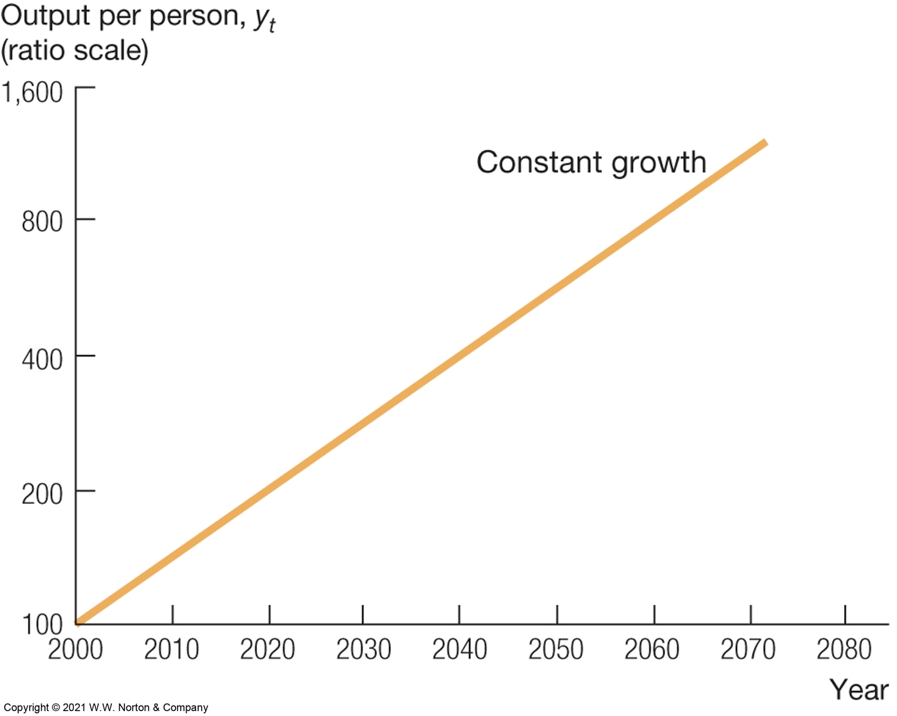
\includegraphics[width=0.5\linewidth]{Figures/output_per_person}
	\end{figure}
	
\end{frame}

\begin{frame}[wide]{Why Is There Growth in the Romer Model}
	The Romer model produces long-run growth
		\begin{itemize}
			\item Does not have diminishing returns to ideas because they are nonrivalrous
			\item Together, labour and ideas have increasing returns 
			\item Returns to ideas are unrestricted -- R\&D leads to sustained growth of income over time
			\item As the economy accumulates new ideas, the returns to knowledge does not fall (i.e., no depreciation)
			\begin{itemize}
				\item In the Solow model, capital has diminishing returns, capital and income stop growing eventually
			\end{itemize}
		\end{itemize}
%		\item In the Solow model, capital has diminishing returns, capital and income stop growing eventually
%		\begin{itemize}
%			\item The distinction between goods that are objects and ideas allows for long-run growth that capital and labour in the Solow model do not have
%		\end{itemize}
	
\end{frame}

%\begin{frame}[wide]{Balanced Growth}
%	\begin{itemize}
%		\item In the simple Solow model, we have transition dynamics
%		\item In the Romer model, it 
%		\begin{itemize}
%			\item Does not exhibit transition dynamics
%			\begin{itemize}
%				\item The growth rate is constant at all points in time (i.e., growth rate never rises or falls)
%			\end{itemize}
%			\item Instead, has balanced growth path
%			\begin{itemize}
%				\item In some sense the economy could be said to be in its steady state from the start, but it is odd to call this a steady state... we called this balanced growth path
%			\end{itemize}
%			\item Constant growth rates of all endogenous variables
%			
%		\end{itemize}
%	\end{itemize}
%\end{frame}

\begin{frame}[wide]{Case Study: A Model of World Knowledge}
	\begin{itemize}
		\item The United States has more researchers than Luxembourg has people
		\item According to the Romer's model, the growth rate of GDP per capita in the model is tied to the number of researchers
		\begin{itemize}
			\item Therefore, the model would predict that the United States should grow faster than Luxembourg
		\end{itemize}
		\item Between 1960 and 2017,
		\begin{itemize}
			\item U.S. growth rate of per capita GDP: 2.0 percent per year
			\item Luxembourg growth rate of per capita GDP: 2.7 percent per year
		\end{itemize}
		\item All countries can benefit from all ideas, no matter where the ideas were discovered
		\begin{itemize}
			\item e.g., International trade, multinational corporations, licensing agreements, international patent filings, the migration of students and workers, and the open flow of information 
		\end{itemize}
	\end{itemize}
\end{frame}

\begin{frame}[wide]{Experiment: An Increase in Population}
	\begin{itemize}
		\item What happen if a country suddenly one time increase its population? In BGP, ...
		
	\[y_t^* = \left(\frac{1}{\bar{n}}\right)^\gamma \bar{z}^\gamma  (1-\bar{\ell}) \left( \textcolor{blue}{L_{a,t}}\right)^\gamma = \left(\frac{1}{\bar{n}}\right)^\gamma \bar{z}^\gamma  (1-\bar{\ell}) \left( \ell \textcolor{blue}{N_t} \right)^\gamma \]
	\[	g_y^* = \gamma \bar{n} \]
	
		\item Changes in the population can be interpret as an exogenous increase in $N_t$ 
		\begin{itemize}
			\item A larger population means there are more researchers (i.e., $L_a$ increases) lead to more idea being created, so the higher per capita output
		\end{itemize}
		%\item This change the growth rate of idea, $\bar{g}_A$
		\item But, there is no change to $g_y$
		\item Therefore, an increase in population permanently raises per capita output, but after the rise, the growth is the same as before
	\end{itemize}
\end{frame}

\begin{frame}[wide]{Experiment: An Increase in Population}
	\begin{itemize}
		\item What happens during the period before reaching BGP?
		\vspace{1mm}
		\item The economy will follow the transitional dynamics as discussed in the previous chapter. Why does this occur in the Romer model?
		\vspace{1mm}
		\item In the initial period, $y_t$ remains unchanged.
		\begin{itemize}
			\item Recall $Y_t = A_t^\gamma L_{y,t}$. $Y$ increases due to the rise in workers in the production sector (i.e., $L_{y,t} = (1-\ell)N_t$)
			\item In our specification, this cancels out the effect of the increase in $N$, resulting in no immediate change in $y_t$ (i.e., $y_t = A_t^\gamma (1-\ell)$)
		\end{itemize}
	\end{itemize}
\end{frame}

\begin{frame}[wide]{Experiment: An Increase in Population}
	\begin{itemize}
		\item Some of the new population will enter the research sector, accelerating the rate of idea creation (i.e., $\Delta A_{t+1} = \bar{z} L_{a,t} = \bar{z} \ell N_t$).
		\vspace{1mm}
		\item As $A_{t+1}$ increases, $y_{t+1}$ will grow at a faster rate than the increase in $N_{t+1}$ would suggest, leading to a faster rise in $y$
		\vspace{1mm}
		\item This accelerated growth will eventually slow as the $g_A = \frac{\bar{z}L_{a,t}}{A_t}$ returns to the rate of $\bar{n}$ on the BGP 
	\end{itemize}
\end{frame}


%\begin{frame}[wide]{An Increase in Population }
%	\begin{itemize}
%		\item Consider a one-time, permanent increase in the population, $\bar{L}$ in the year 2030
%		\item The growth rate in the Romer model immediately and permanently rises
%	\end{itemize}
%	\begin{figure}
%		\centering
%		\includegraphics[width=0.6\linewidth]{"Figures/An Increase in population"}
%	\end{figure}
%	
%\end{frame}



\begin{frame}[wide]{Growth Effects versus Level Effects}
	\begin{itemize}
		\item Growth effects: changes to the rate of growth of per capita output
		\begin{itemize}
			\item Changes that affect $g$'s
		\end{itemize}
		\vspace{3mm}
		\item Level effects: Changes in the level of per capita GDP
		\begin{itemize}
			\item Changes affect $y$, $Y$, and so forth
		\end{itemize}
		
%		\item Growth effects are eliminated if the exponent on ideas is less than 1,
%		due to diminishing returns
%		\begin{itemize}
%			\item More researchers produce more ideas, and this raises the long-run level of per capita GDP
%		\end{itemize}
	\end{itemize}
\end{frame}

%\begin{frame}[wide]{On the Possibility of Progress}
%	Can economic growth be sustained given that we live on a planet with finite resources?
%	\begin{itemize}
%		\item Prices of industrial commodities have been falling
%		\item We can see that the industrialization of China and India has made an impact around the year 2000
%	\end{itemize}
%	\begin{figure}
%		\centering
%		\includegraphics[width=0.5\linewidth]{"Figures/On the Possibility of Progress"}
%	\end{figure}
%	
%\end{frame}
%
%\begin{frame}[wide]{On the Possibility of Progress}
%	\begin{itemize}
%		\item A standard supply-and-demand analysis might go like this: 
%		\begin{itemize}
%			\item Commodities are in finite supply
%			\item There is a massive increase in the demand for these resources
%			\item Increases in demand combined with a fixed supply is a recipe for enormous increases in price
%		\end{itemize}
%		\item Our story about demand is surely correct: 
%		\begin{itemize}
%			\item It turns out that rather than being finite, supply must have expanded by even more than demand 
%			\item We found new supplies of these resources and discovered new technologies for extracting 
%			\item We discovered new ways to use these resources more efficiently
%		\end{itemize}
%		\item On net, these supply forces evidently outweighed the massive increases in demand during the twentieth century, leading to large overall price declines
%	\end{itemize}
%	
%\end{frame}

%\begin{frame}[wide]{An Increase in the Investment Rate}
%	\begin{columns} 
%			% Column 1
%			\begin{column}{.5\textwidth}
%				\begin{itemize}
%					\item Suppose the investment rate increases permanently for exogenous reasons ($s'>s$)
%					\begin{itemize}
%						\item The investment curve rotates upward ($\bar{s}'\bar{A}  \bar{L}^{1-\alpha} K_t^\alpha > \bar{s}\bar{A}  \bar{L}^{1-\alpha} K_t^\alpha$)
%						\item The depreciation curve remains unchanged ($\delta K_t$)
%						\item The capital stock increases by transition dynamics to reach the new steady state
%						\begin{itemize}
%							\item This happens because investment exceeds depreciation ($sY_t>\delta K_t$)
%						\end{itemize}
%						\item The new steady state is located to the right
%					\end{itemize}
%				\end{itemize}
%			\end{column}
%			% Column 2    
%			\begin{column}{.5\textwidth}			
%				\begin{figure}
%					\centering
%					\includegraphics[width=1\linewidth]{"Figures/An Increase in the Investment Rate"}
%				\end{figure}
%			\end{column}%
%		\end{columns}
%\end{frame}

%\begin{frame}[wide]{Measuring the State of the Economy}
%	\begin{columns} 
%		% Column 1
%		\begin{column}{.5\textwidth}
%			\begin{table}[htbp]
%				\centering
%				\begin{tabular}{lrrrr}
%					& 2005  & 2006  & 2007  & 2008 \\
%					\hline
%					GDP   & 12.6  & 13.4  & 14.0    & 14.3 \\
%					(in trillions of \$) &       &       &       &  \\
%					Growth rate GDP &       & 0.063 & 0.045 & 0.021 \\
%					\hline
%				\end{tabular}%
%				\label{tab:addlabel}%
%			\end{table}%
%		\end{column}
%		% Column 2    
%		\begin{column}{.5\textwidth}			
%			
%			
%		\end{column}%
%	\end{columns}
%\end{frame}

\begin{frame}[wide]{Next Lecture}
	\begin{itemize}
		\item Next lecture will finish Ch.6
	\end{itemize}
\end{frame}

\end{document}